\section{"2" Определение физико-механических свойств поверхности}

\begin{frame}[t]{Определение физико-механических свойств}
\framesubtitle{}
    \small
    Определить процентное соотношение твердых, упругих и пластичных свойств пройденной поверхности

\textbf{Метод решения}: машинное обучение, Метод Опорных Векторов (SVM) 

\textbf{Идея решения}: Создается установка для обучения. Обучение: робот ходит по различным типам поверхностей фиксированное количество касаний поверхности с постоянной угловой скоростью. Собранные данные разбиваются на 2 части 80\% и 20\%. Модель обучается на 80\% с помощью ядра PUK7. Тестирование: происходит на оставшиеся 20\%.  Используются метрики меткости, точности, полноты и F1-счета.

\begin{columns}[T,onlytextwidth]
    \begin{column}{0.44\textwidth}
        \textbf{Входные данные}: обученный классификатор 
поверхностей, данные с внутренних 
датчиков робота

\textbf{Выходные данные}: процентное 
соотношение упругих, твердых 
и пластичных свойств 
пройденной поверхности

\textbf{Допустимая ошибка}: 20\% - точность

\textbf{Предположения}: 1) На рисунке.

    \end{column}
    \begin{column}{0.54\textwidth}
        \vspace{-0.9cm}
        \begin{figure}[H]
            \begin{subfigure}[b]{0.3\textwidth}
                \centering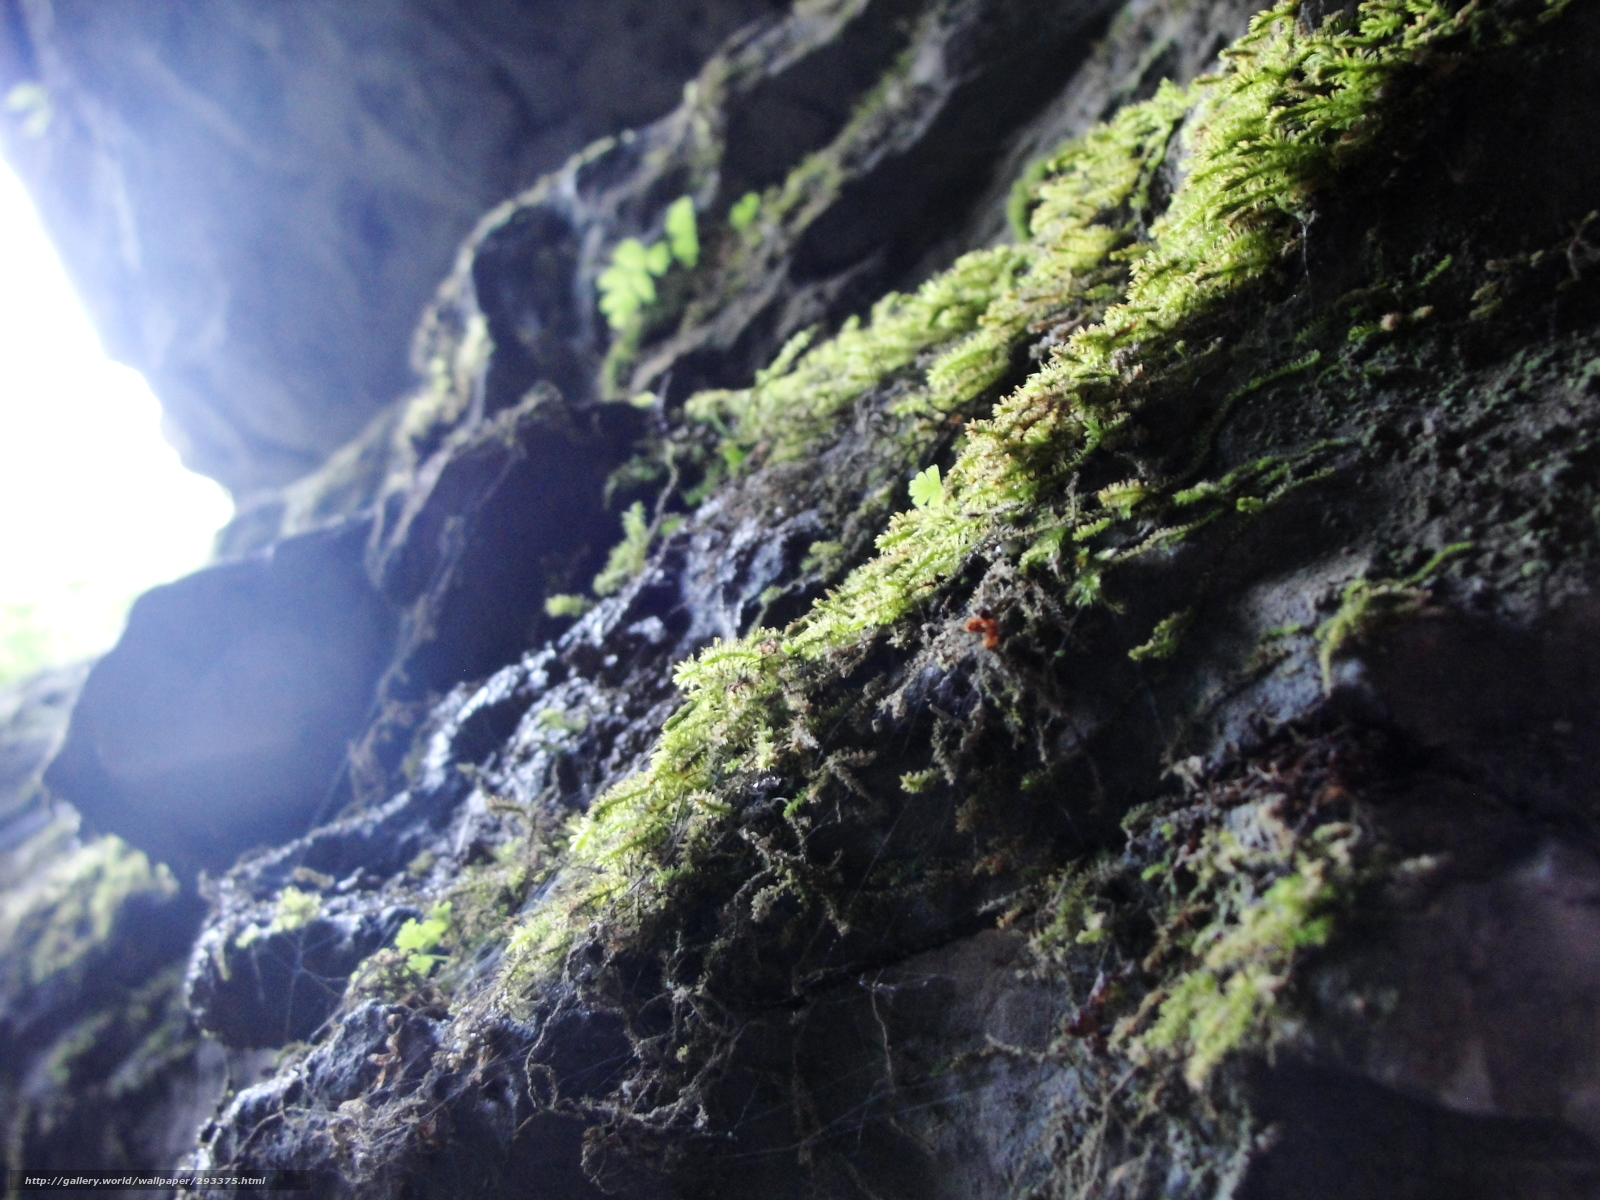
\includegraphics[height=1.5cm,width=1\textwidth,keepaspectratio]{surface_types/moss.jpg}
            \end{subfigure}
            \hfill
            \begin{subfigure}[b]{0.3\textwidth}
                \centering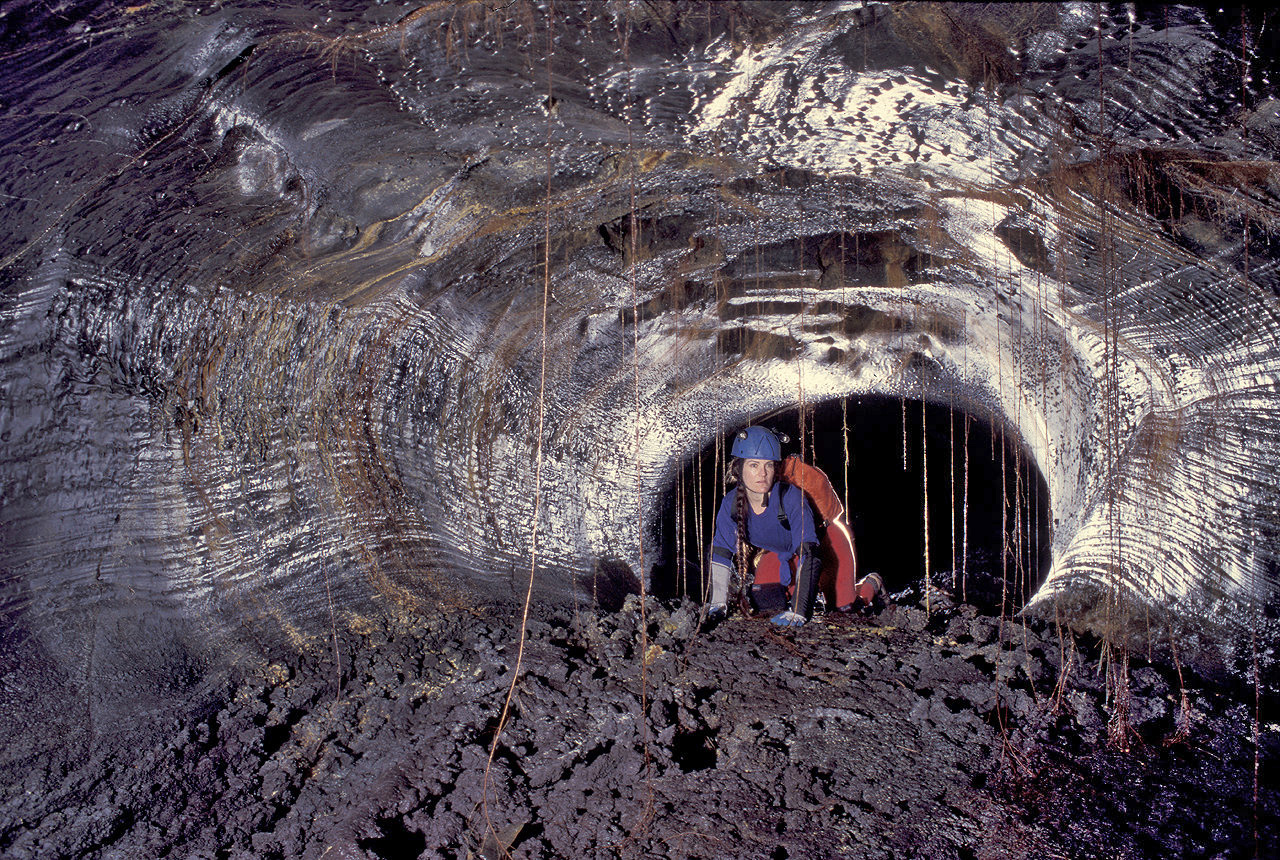
\includegraphics[height=1.5cm,width=1\textwidth,keepaspectratio]{surface_types/lava.jpg}
            \end{subfigure}
            \hfill
            \begin{subfigure}[b]{0.3\textwidth}
                \centering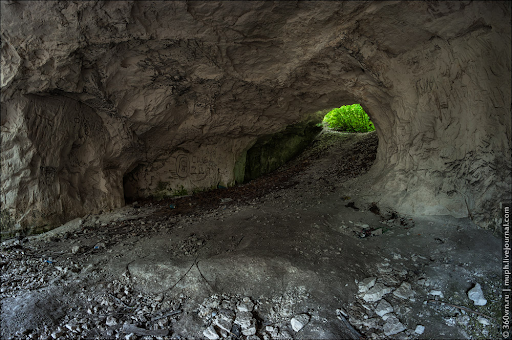
\includegraphics[height=1.5cm,width=1\textwidth,keepaspectratio]{surface_types/moul.png}
            \end{subfigure}
    
            \begin{subfigure}[b]{0.3\textwidth}
                \centering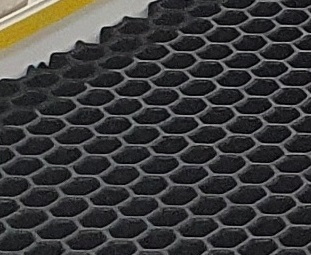
\includegraphics[height=1.5cm,width=1\textwidth,keepaspectratio]{surface_types/rubber.JPG}
            \end{subfigure}
            \hfill
            \begin{subfigure}[b]{0.3\textwidth}
                \centering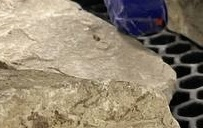
\includegraphics[height=1.5cm,width=1\textwidth,keepaspectratio]{surface_types/rock.jpg}
            \end{subfigure}
            \hfill
            \begin{subfigure}[b]{0.3\textwidth}
                \centering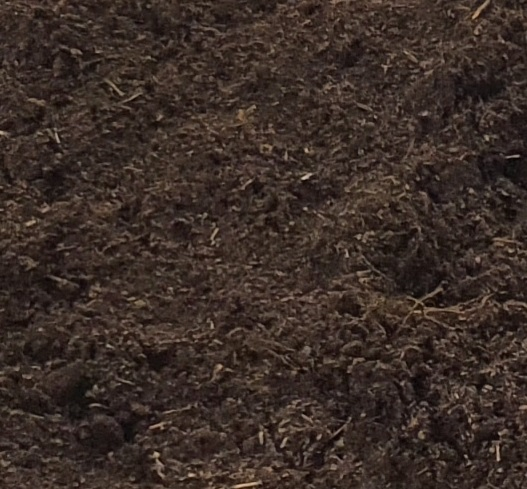
\includegraphics[height=1.5cm,width=1\textwidth,keepaspectratio]{surface_types/zemlya.jpg}\\
            \end{subfigure}
            \vspace{-0.3cm}
            \caption{Эталоны упругой, твердой и пластичной поверхностей}
        \end{figure}
    \end{column}
\end{columns}
\end{frame}

\note{Имея разработанный сенсор и узел с ногой робота, возможно решать задачу определения физико-механических свойств поверхности.

Для получения более точных результатов, было решено решать данную задачу натурно.

Для получения процентного соотношения упругих, твердых и пластичных свойств пройденной поверхности, необходимо обучить модель. Для этого было решено использовать метод опорных векторов (SVM). На рисунке представлены объекты, которые использовались как эталонные упругие, твердые и пластичные поверхности, а также их аналог в пещерах.

Данные для решения задачи классификации собирались так. Робот ходит по различным типам поверхностей фиксированное количество касаний поверхности с постоянной угловой скоростью. Данные с внутренних датчиков, о которых будет разговор далее, собираются. Когда были собраны данные для всех типов поверхностей, то они разбивались на 2 части. 80 процентов использовались для обучения, 20 - для тестирования. Использовались классические критерии для данного типа задачи: меткость, точность, полнота и F1-счет.
}

\begin{frame}[t]{Стенд}
    \framesubtitle{}
    \begin{figure}[H]
        \begin{subfigure}{0.33\textwidth}
            \centering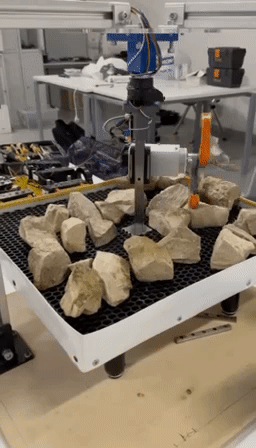
\includegraphics[height=4cm,width=1\textwidth,keepaspectratio]{s_shape_leg/rockk.png}
            \caption{Установка}
        \end{subfigure}
        \begin{subfigure}{0.33\textwidth}
            \centering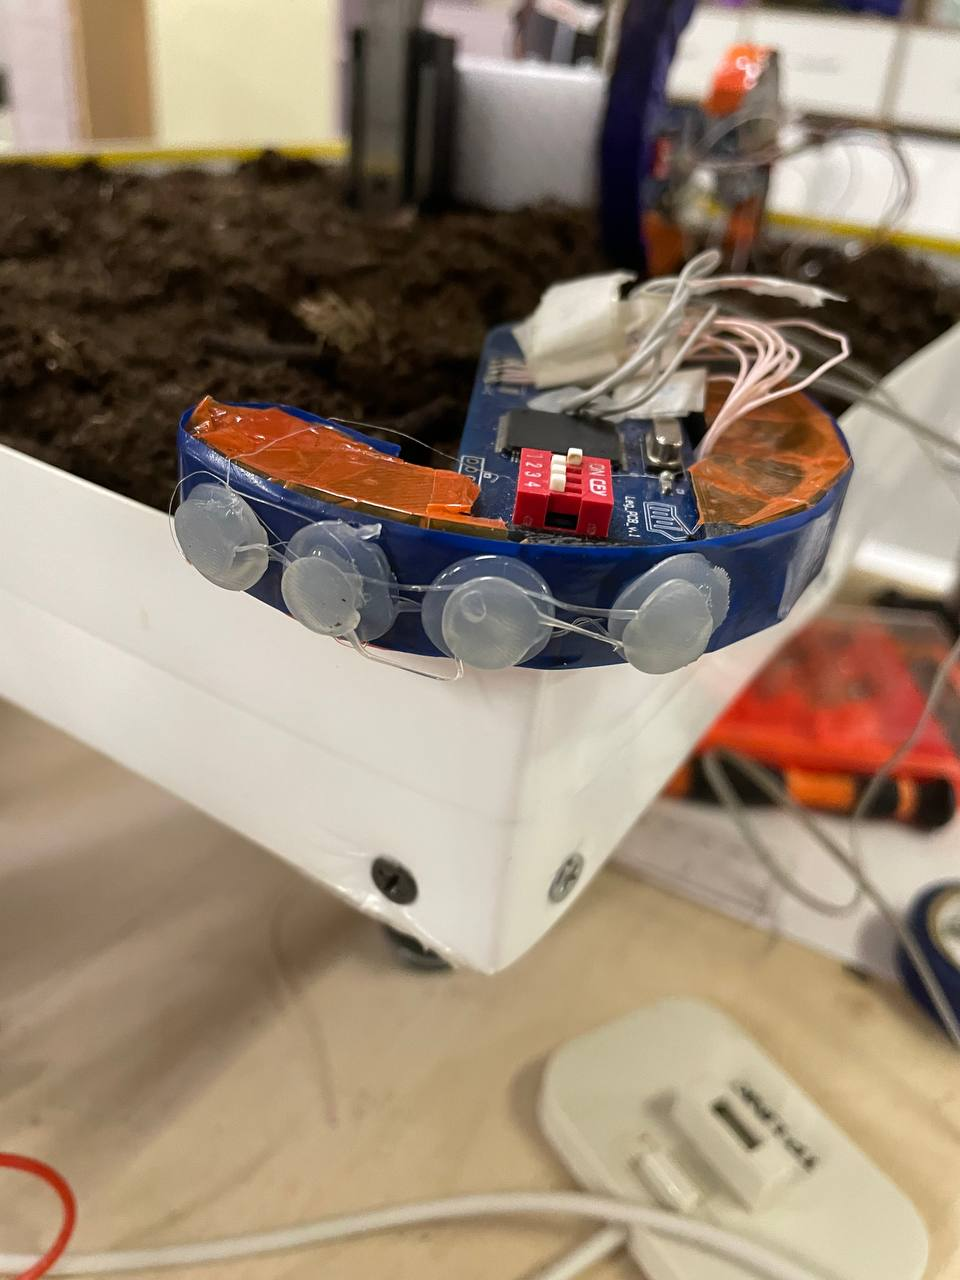
\includegraphics[height=4cm,width=1\textwidth,keepaspectratio]{s_shape_leg/socks.jpg}
            \caption{Нога робота с установленными сенсорами}
        \end{subfigure}
        \begin{subfigure}{0.33\textwidth}
            \centering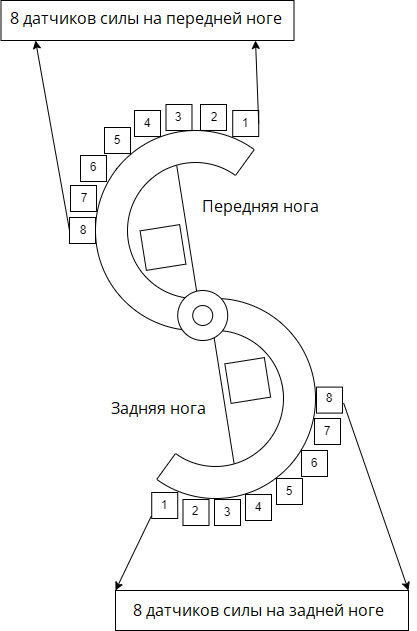
\includegraphics[height=4cm,width=1\textwidth,keepaspectratio]{s_shape_leg/leg_design.png}
            \caption{Схематическое распределение сенсоров на ноге}
        \end{subfigure}
    \end{figure}
\end{frame}

\note{На экране представлен стенд, нога робота, на которую установлены датчики силы, а также способ их установки. Нужно отметить, что во время испытаний, пришел к выводу, что максимум нужно 5 сенсоров, а не 8, как указано на рисунке справа.
}

\begin{frame}[t]{Метод опорных векторов}
\framesubtitle{}
\small
\begin{columns}[T,onlytextwidth]
    \begin{column}{0.49\textwidth}
        \vspace{-0.5cm}
        \begin{align}
            f(x) = w^T x + b
        \end{align}
        где $w$ --- весовой вектор, $b$ --- смещение,

        $x$ --- \textbf{входной вектор}:

        (1) Частота движения ног\\
        (2-6) Пиковая и средняя амплитуда, среднее значение, ширина, площадь под кривой давления с датчика силы\\
        (7-11) Индивидуальная пиковая амплитуда силы для каждого датчика\\
        (12-15) Пиковая и средняя амплитуда, среднее значение, ширина, площадь под кривой  крутящего момента двигателя\\
        (16) Среднее давление на сенсорах
    \end{column}
    \begin{column}{0.49\textwidth}
        Ядро на основе функции Пирсона VII:
\begin{align}
    K(x, y) = (1 + ((||x - y||^2)/\sigma^2)^\omega)^{(-1/\omega)}
\end{align}
Где $x$, $y$ --- векторы во входном пространстве, $||x - y|||$ --- евклидово расстояние между $x$ и $y$, $\sigma$ --- масштабный параметр, определяющий <<разброс>> ядра, $\omega$ --- это параметр формы, который влияет на форму границы принятия решения.

\begin{figure}[H]
    \begin{subfigure}{0.49\textwidth}
        \centering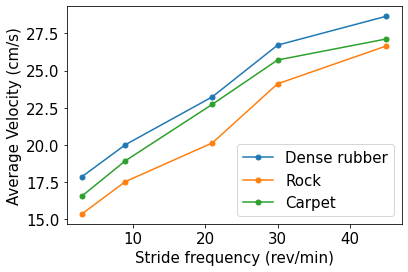
\includegraphics[height=2cm,width=1\textwidth,keepaspectratio]{../images/s_shape_leg/avg_lin_vel_rev_min.png}
        \caption{График}
    \end{subfigure}
    \begin{subfigure}{0.49\textwidth}
        \centering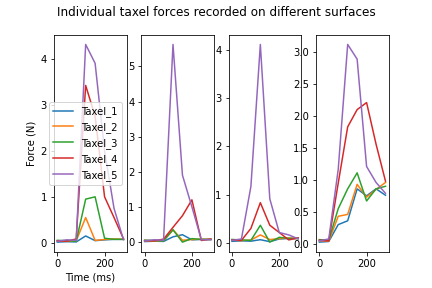
\includegraphics[height=2cm,width=1\textwidth,keepaspectratio]{../images/s_shape_leg/TaxelIndForce.png}
        \caption{Таксель}
    \end{subfigure}
\end{figure}
    \end{column}
\end{columns}
\end{frame}

\note{Метод опорных векторов описывается следующей формулой. Входной вектор включал в себя частоту движения ног, так как показано на рисунке справа - он может критерием определения. Информация с датчиков силы, а также с мотора - основные показания.

Функция ядра обычно преобразует обучающий набор данных таким образом, что нелинейная поверхность принятия решений способна преобразовываться в линейное уравнение в пространствах большего числа измерений. Для этого использовалась функция Пирсона VII.
}

\begin{frame}[t]{Результаты}
    \framesubtitle{}
    \begin{figure}[H]
        \begin{subfigure}{0.49\textwidth}
            \caption{Таблица}
            \resizebox{\linewidth}{!}{%
                \begin{tabular}{|c|c|c|c|c|}
                    \cline{3-5}
                    \multicolumn{1}{l}{}                     & \multicolumn{1}{l|}{} & \multicolumn{3}{c|}{\textbf{Предсказанный класс}}                                                                                           \\
                    \cline{3-5}
                    \multicolumn{1}{l}{}                     &                       & Камень                                            & Резина                                     & Земля                                      \\
                    \hline
                    \multirow{3}{*}{{\textbf{Истин. класс}}} & Камень                & {\cellcolor[rgb]{0.741,0.843,0.929}}84.0\%        & 2.56\%                                     & 13.44\%                                    \\
                    \hhline{|~----|}
                                                             & Резина                & 20.1\%                                            & {\cellcolor[rgb]{0.741,0.843,0.929}}67.8\% & 12.1\%                                     \\
                    \hhline{|~----|}
                                                             & Земля                 & 1.0\%                                             & 18.9\%                                     & {\cellcolor[rgb]{0.741,0.843,0.929}}80.1\% \\
                    \hline
                \end{tabular}
            }
        \end{subfigure}
        \begin{subfigure}{0.49\textwidth}
            \centering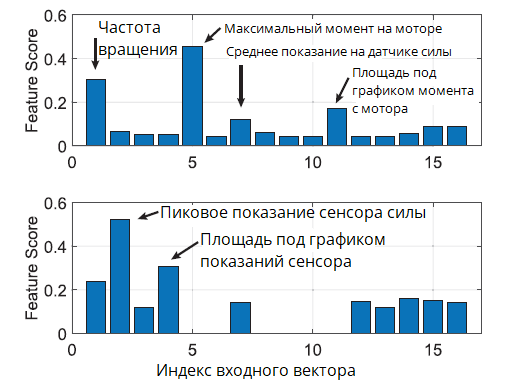
\includegraphics[height=4cm,width=1\textwidth,keepaspectratio]{../images/s_shape_leg/feature_score.png}
            \caption{Feature score}
        \end{subfigure}
    \end{figure}
\end{frame}

\note{Справа представлено
}